\chapter{MIWWG:支配者の存在しないIoTデータ市場}
本章では、本研究で提案するIoTデータ市場であるMIWWGについての要件と、そのデータ市場における取引のプロセスについて記述する。
また、MIWWGとは "MIWWG works without governor"を表し、再帰的頭字語を使っている。

\section{MIWWGが達成する目的}
本研究の最終的な目標はオープンなIoTデータ市場の参加者が、参加者自らの意思によってルールや管理団体を設立できるものである。
詳細な理由については4.2.1項にて後述するが、今のクローズドなIoTデータ市場の方式を拡張することでこの理想の実現を目指すことは難しい。
一方で、オープンなIoTデータ市場の方式を拡張することでこの理想の現実を目指すことは可能であると考える。
この時、もっとも最終的な理想の市場を実現するため、もっともオープンな市場を実現することが本研究のMIWWGが達成する目的である。
今後このP2P通信によって構築されたMIWWGを基にした、ルールや管理団体の設立の方法について議論や実装が行われることを期待するものである。

\section{市場の要件}
本節では、前節に記述した達成する目的のため、より具体的に市場が満たすべき要件を述べる。
前半の1~2項に関しては機能要件であり、後半の3~6項に関しては非機能要件である。
前半はMIWWGの基本理念を継承したものであるか否かを測るものとして、後半はMIWWGの評価指標としてMIWWGが改良されて行くこの先も使用されうるものであることを意識して記述した。

\subsection{中央集権装置を必要としない通信モデルによる市場の創造}
本市場において、中央集権組織である管理者の存在はオープンな市場である上でもっとも不要なものである。
管理者は市場を一存で動かせるため、当然ながら巨大な力を持ち得る。
そしてこの大きな力は市場の前提条件を簡単にひっくり返せたり、市場の取引に対する疑義を生じさせる原因となる。
全員が透明に見ることが可能なルールによる支配を行えることにより、この危険性への懸念や疑義を払拭することが出来る。
この中央集権組織支配の排除を目指すとき、既存の代表的なサービス提供方式であるサーバ・クライアント型ではサーバ上でサービスが提供される以上、このサーバの管理者が市場に管理者となってしまい目標の達成が難しい。
そこで例えばP2P通信により、市場の参加者の全員が対等な立場で市場を形成することを考える。
P2P通信は特定の管理者を不必要とするが、このP2P通信上で同意を得た上で管理者にあたるノードを選ぶことは可能である上、P2P通信上でルールやプロトコルを作ることは可能である。
ここで規制が丁度良いルールや管理団体の存在する市場を目指すとき、もっともクライアント・サーバ型を使ったクローズドな市場から目指すことは難しいが、逆にP2P通信型を使ったオープンな市場から目指すことは可能であるという現状が見えてくる。
そしてMIWWGは丁度良い規制の市場を目指す最初の段階として、もっともオープンでルールも管理団体も存在しないIoTデータ市場をP2P通信で実現することを目的としている。
よってMIWWGの機能要件の一つとして、P2P通信を始めとした中央集権装置を必要としない通信モデルによる市場の創造が挙げられる。

\subsection{データの売買}
本市場において、データの売買が可能である必要がある。
ここで売買とは何かを日本国の民法555条から引用して考える。
「売買は、当事者の一方がある財産権を相手方に移転することを約し、相手方がこれに対してその代金を支払うことを約することによって、その効力を生ずる。」
つまり、データ売買に関する取引が成立したとき、データの売り手が買い手へデータを提供する必要がある。
また同時に、買い手は売り手へ代金を支払う必要がある。
そして、これらには契約と同時に上記二つの必要な要件を履行する義務が生じる。
但し、これらは法律的な売買の定義とその解釈であり、実際にデータの売買契約には以下のプロセスが必要となる。
また、今後そのプロセスを遂行するために作られたモジュールを呼ぶための名称を付記する。
\begin{enumerate}
\item 売り手がどのようなデータを売りたいか、またその値段などを示し、データを出品する。データ出品モジュール
\item 買い手が出品されたデータを閲覧する。:出品データ一覧取得モジュール
\item 買い手が閲覧したデータの中から欲しいデータを選び、売り手へ売買契約を申し込む。:売買申し込みモジュール
\item 売り手は申し込まれた契約に対し、応じるか否かの返答をする。:売買契約前確認モジュール
\item 売り手が申し込みに応じた場合、売買契約を成立させる。:売買契約作成モジュール
\item 買い手が売り手へ代金を支払う義務を遂行させる。:支払い義務遂行モジュール
\item 売り手が買い手へデータを転送する義務を遂行させる。:データ転送義務遂行モジュール
\end{enumerate}
以上が必要なプロセスであり、データの売買に必要な要件である。

\subsection{取引に関する秘匿性}
ここでは2点について述べる。
A. データに関して、売り手が意図しない相手へのデータの公開は行わない。
B. 取引の内容について、トークンやデータの取引上必要な情報以外は極力ブロックチェーン上に載せず、公開しない。
まずAについてだが、データは情報商品であり、その情報は一般に入手できないため、価値が存在するものである。
そのデータが本市場の上から意図しないところへ大量に漏れるとすれば、それは本市場がデータの価値を毀損していることにつながり、本市場が意味の少ないものになってしまう。
よってブロックチェーン上へデータを送るなど、マイナーを含む買い手以外の人間に対して売り手が意図しないところでデータが公開されることは避けなければならない。
次にBについてだが、例えばデータを取得するためのアクセス先かアクセス元を公開しなければならないとする。
例えばデータを売り手が買い手へプッシュするのか、買い手が売り手にプルするのかについて議論をしてみる。
この時http(s)通信を使い、 curlなどでデータをプッシュかプルをする際は必ず売り手か買い手がIPアドレスをブロックチェーン上へ暴露しなければならない。
そうでなければ、ノードが見つからないためだ。
ここでは平均して1つの事業者が平均でm個のデータノードを所有しており、1つのデータノードは平均してn個の事業者にデータを売ると考えられる市場を仮定する。
この時、データ受け取り手のIPアドレスを暴露する場合は1人の事業者に対して\(m \times n \)個のIPアドレスを暴露する必要がある。
一方でデータの送り手のIPアドレスを暴露する場合は1人の事業者に対して \(\frac{1}{ m \times n }\)個のアドレスを暴露する必要がある。
するとこの場合、\(m \times n \ge 1\)であればデータの送り手のIPアドレスを暴露する方が、事業者に紐付く情報が少なく済む可能性がある。
勿論、これに関しては作成する市場の目的によって異なる。
また、IPアドレスよりも一時的に使用するために生成されたメールアドレスなどの方が、より秘匿性は高い場合も存在するであろう。
ここでは、取引に関してなるべく他者から秘匿されるべき項目についてあげ、記述を行なった。

\subsection{売買方法の決定可能性}
オープンでルールや支配組織の存在しない市場は、売り手が広場に農作物を持ち寄って勝手に出来上がる市場と同じようなものである。
そこにおいては当然、売り手は好きな方法で好きな値段をつけて商売ができる。
これと同じように、本市場の売買方法はフレキシブルである方が良い。
例えば4.2.2項で記した「支払い義務遂行モジュール」と「データ転送義務遂行モジュール」の二つについて考えてみる。
民法による売買の定義を参照すると、本来は売買契約と同時に、売主の財産権移転義務と買主の代金支払義務は同時履行される。
しかし、データとトークンを同時に一瞬のラグもなく送信し合うことは技術的に難しい。
そこでデータとトークンのどちらを先に送信するかについて議論が起こる。
売り手のデータの到着を確認して、買い手のトークンを送るのか、あるいはその逆か。
後払いを選んだ場合、最初に売り手がデータを投げ、それに対して買い手は支払いを行う。
その後はトークンの移動を売り手が確認してから新しくデータを投げることとなる。
一方で前払いを選んだ場合、最初に買い手がトークンを投げ、それに対して売り手はデータを送る。
その後は買い手は送られてきたデータを確認してから新しいトークンを投げ、必要なデータを取得することとなる。
前払いが良いか後払いが良いかは、売るべきデータの種類に依存すると考えられる。
例えば3秒に1回送信されるデータであり、データが何個も連続して時系列に送られることによって初めて価値のあるデータというものが存在するだろう。
例えば高速道路を定点観察している写真がこのデータの内容である場合だ。
この時は、データに対して後払いを認めた方が得であると考えられる。
何故なら、ユーザはそのデータの内容を見てから、本当に欲しかったデータ形式やデータ内容であるかを精査できるからである。
一方。例えばある地点の気温と湿度のデータを10分に1回送信しているデータノードが存在するとしよう。
この時に後払いを認めてしまうと、一度しか情報が入らない人は常に一度のみのデータを貰い、それに対するデータを払わずに取引を中断してしまう可能性がある。
このように、前払いか後払いかについてでも、データの内容によって売り手の希望は変わってくる。
同じように、何個のデータに対してどれだけのトークンを支払い、支払いのラグはどこまで認めるのかについて売り手がよりフレキシブルに決められることが要件の一つである。

\subsection{大量なIoTデータのリアルタイム処理}
本研究において、IoTデータとは細かい間隔(1~10秒)でリアルタイム流れてくるデータのことを呼ぶ。
蓄積データが対となる概念であり、ある都市の過去1年間の気温データなどはリアルタイムではなく既に存在しているデータであるので、蓄積データと呼ぶ。
これに対し、現在のある都市の気温はリアルタイムで取得できるデータであり、IoTデータと呼ぶ。
このIoTデータの売買を裁くには、大量の処理を裁く必要が出てくる。
少なくとも、PoW(Proof of Work)を基にしたブロックチェーンのオンチェーン技術のみでは裁くことができない。
その場合はオフチェーンを利用することが考えられる。
また、将来的には一部をオンチェーンでPoA(Proof of Authority)を利用し、一部の管理団体がトランザクションを速く裁くことも必要になるかもしれない。
PoAとはトランザクションのマイニングを一部の有資格者が行える仕組みのことで、一定のハッシュパワーでトランザクションの承認が行われる方式である。
この方式は、承認者の数が多いほど捌けるトランザクションの数が増えるという利点を持っている。
一方で、中央集権型の統治へ逆戻りしてしまっている様子も伺える。
オンチェーンやオフチェーン\UTF{00B7}それに関わる政治的な要素は様々あるが、IoTデータというリアルタイムデータを扱う以上、大量データのリアルタイム処理を行えることは要件の一つである。

\subsection{ダウンタイムの非存在}
IoTデータ市場はIoTの発展に伴い、とても大きな市場規模を持つようになる。
データ市場に限らない数値であるが、2022年のIoT市場規模は11.7兆円と言われている。(http://www.itmedia.co.jp/enterprise/articles/1809/13/news132.html)
このようなプラットフォーム上で大きな価値のあるアプリケーションが動いている場合は、ダウンタイムが起きると多額の損害が生まれてしまう。
その状況の中で、2章で述べたようにAWSのSLAは99.99\%であり、年間では52.56分落ちている可能性があるのだ。
そのわずか一時間弱の間であっても、IoTデータ市場の規模の大きさを考えるとダウンタイムは看過できない。
また機械的のハードウェア的な故障のみならず、人為的なバグや人為的なオペレーションミスも一つのサーバ上でサービスが動いている場合は考えうる。
そこでP2P通信を始めとした方法で、ある事業者のサーバが壊れてもネットワーク全体には影響を及ぼしにくいサービスモデルであることが望ましい。
P2P通信であることは要件にはならないが、ダウンタイムの存在がほぼ否定されるほど、この市場が動くネットワークがダウンタイムを起こしにくくすることは要件の一つである。

\section{取引のプロセス}
本節では、MIWWGにおけるIoTデータ取引のプロセスを示す。

\subsection{データ陳列}
最初に、データの売り手が自分の持っているデータの種類をMIWWGネットワーク上へ公開する。
この際、取引に必要な事項である値段やデータが送信される間隔といった値を同時に提出する。
しかしデータについての詳細な説明書きや例を大量の文字によって記述する場合があった場合、マイナーへ大きな量の手数料を払う必要が生じる。
その際はデータに関する詳細を記述したURLを記述し、そのURLに詳細なデータに関する記述を行うという方法を取ることも可能である。
売り手は自身の持つデータをブロックチェーン上へと送信し、これがブロックに含まれた瞬間からデータが全ノードへと知れ渡ることとなる。

\subsection{取引開始}
次に、買い手が陳列されたデータを閲覧し、必要なデータについて取引を開始する。
この時、一般的なオフチェーン技術の特徴から、買い手は今後どの程度の期間でそのデータが必要であるかについて考慮し、その期間の間に使われる分のトークン量をデポジットする必要がある。
このデポジットについては、相手の同意のない限りデータの買い手側が即座に引き出すことはできない。
取引開始のトランザクションをブロックチェーン上へ送信し、それがブロックに含まれた瞬間が取引開始の瞬間である。
トランザクションがブロックに含まれた後、http(s)通信などによってデータを読み込む際のIDとパスワードをデータの販売元へ送信する必要がある。

\subsection{データ販売とトークン転送}
本項を含む、オフチェーンの文脈においてトークンの転送とは、買い手がそのトークンバランスに同意したことを示す署名値を売り手へ送信することである。
取引開始後、トークンが買い手から売り手へとデータの送信間隔と同じ間隔で送信される。
データ転送を売り手が止めた場合、買い手はトークンの転送を止める。
逆に、トークンの転送を買い手が止めた場合は、売り手はデータ転送を止める。
この際、故意に転送を止めた場合でなくとも、ネットワークの一時的な不通によってデータやトークンの転送が行われなかった場合も同様に相手側は取引を停止する。
従って、データ陳列の際にどの程度の支払いの遅れまでを売り手が許容するかという内容や、売り手のネットワーク状況によってどの程度のデータ転送の遅れまでを買い手が許容するかという内容についてをデータ陳列の際に記述しておくべきである。
このデータ転送はhttp(s)通信によって行われ、ブロックチェーンネットワークとは全く関係のない動きをする。
従って、これらのデータ販売や転送はブロックチェーンの処理能力に囚われない。

\subsection{取引終了}
買い手がトークンの転送をやめた場合や売り手がデータの転送をやめた場合は取引の途中であっても取引が終了する場合がある。
逆に、デポジットの全ての転送が終わった場合はデータの売り手によって取引は終了される。
いずれでも、買い手か売り手が取引終了に関するトランザクションがブロックチェーンネットワークに送信することで、取引は終了を迎える。

\section{まとめ}
本章に記述したプロセスを一つの図で示したものが以下の図\ref{process}である。
買い手と売り手がどちらも取引終了を主張した場合のプロセスを示している。
\begin{figure}[htbp]
 \centering
  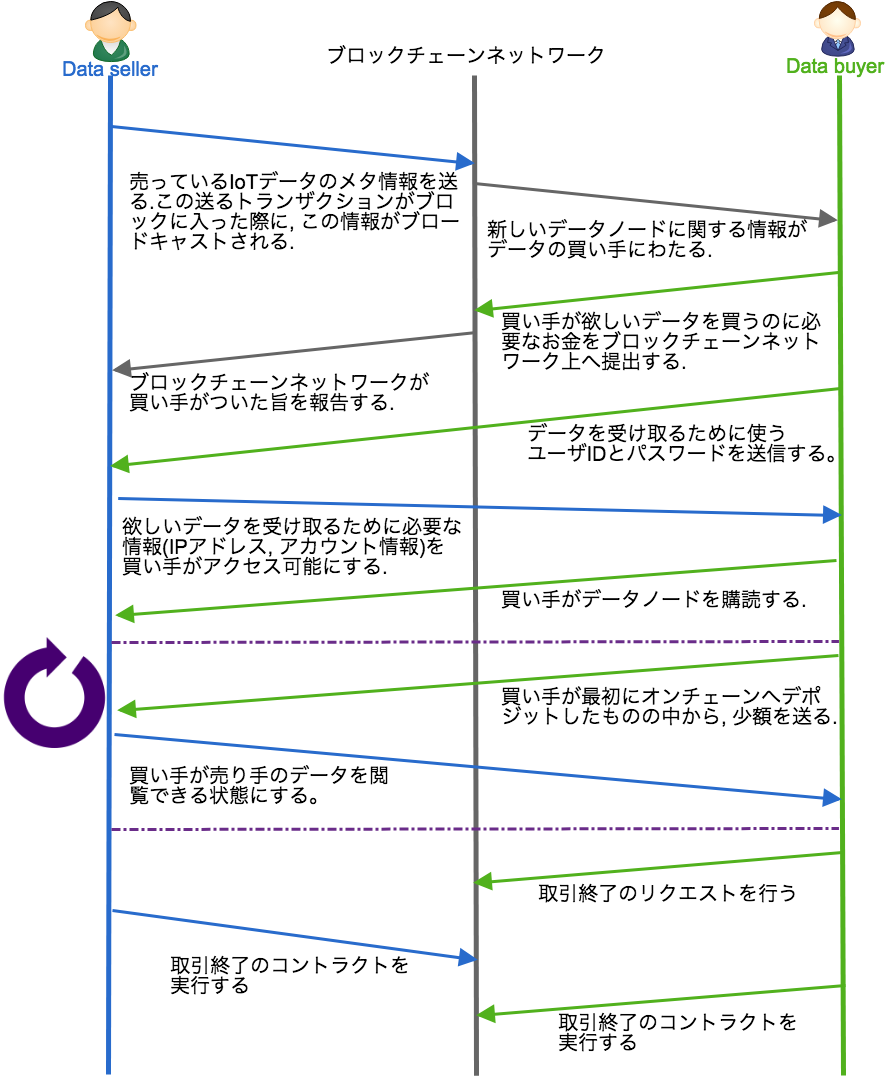
\includegraphics[width=140mm]{image/process.png}
 \caption{MIWWGの取引プロセス}
 \label{system}
\end{figure}

